\chapter{Simulation}

\label{chap3}
As discussed in previous chapter, we implemented MSFC in ns-3 to see how well it performs in simulated conditions and compare it to other traffic schedulers for the benchmark. We simulate a part of Wi-Fi network infrastructure similar to networks of wireless-based Internet providers, which is the environment targeted by the scheduler. We compare the MSFC to 3 other traffic schedulers: CoDel, FQ CoDel and pfifo\_fast. In each run, we install the benchmarked scheduler on all network interfaces of all nodes in the network.

\section{Simulation testbed}
\label{testbed}
\begin{figure}
	\centering
	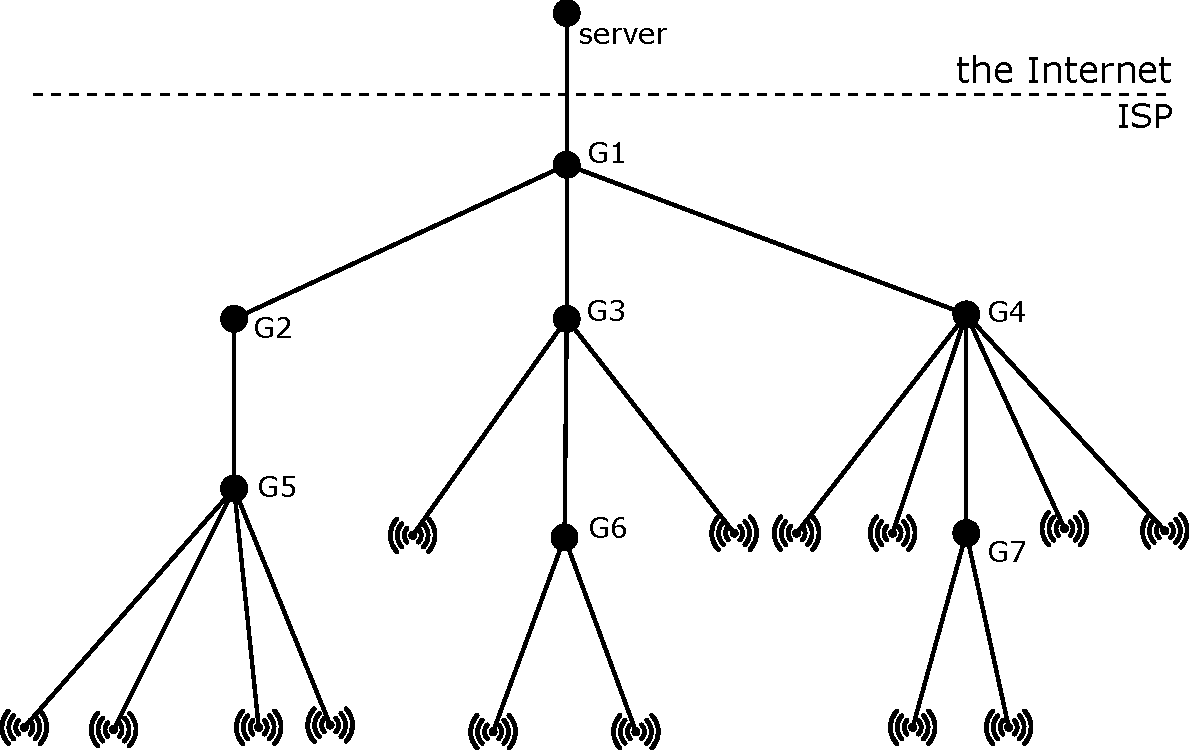
\includegraphics[width=137mm]{drawings/layout}
	\caption{The simulated network topology}
	\label{fig11:sim_layout}
\end{figure}


The simulated network is illustrated in Figure \ref{fig11:sim_layout}. The network is tree-shaped. The topmost node is server that serves as the rest of the Internet. Further, there is part of the infrastructure of an ISP. There are gateway nodes G1-G7. All gateways have 2--5 children. The leafs of this tree are access points (APs) of wireless networks. Finally, 8--12 clients (customers of ISP) are connected to each AP, this results in total of 140 clients.

Each client is connected to exactly one AP. The clients are connected with 802.11ac Wi-Fi --- they share the Wi-Fi bandwidth. APs and gateways are connected with point-to-point links with 100Mbps bandwidth and 5ms delay. The server is connected to the root node G1 of the tree using 1000Mbps link with 50ms delay.

The clients download and upload data. All the traffic flows between the server and the clients. There are several types of flows that model various behaviours of real-world Internet users. The types are listed in table \ref{tab:traffic}. They vary in transport protocol used, size of a single packet and the data rate at which they generate traffic. The data rate may be constant --- in that case the application generates packets on regular basis (e.g. it sends a packet every 5 milliseconds), or it may be variable.

The applications with variable bit rate turn on and off on irregular basis. When switched off, it does not send any packets and when switched on it sends packets at configured constant rate. The on and off durations are generated randomly --- using normal distribution $\mathcal{N}(1,1)$ bound to interval~$\left\langle0,2\right\rangle$.

The count ratio column specifies the ratio of number of applications installed per type. The values in the Table \ref{tab:traffic} mean, that there are 20 times more \emph{HTTP} flows than \emph{SSH} flows. We set the total number of applications to 280 --- 2 applications are installed on every client. 

\begin{table}
	\centering
	
	\begin{tabular}{@{}lllllll@{}}
		\toprule
		Name     & Protocol & Data rate & C/VBR & directions & Packet  & Count \\
		         &          &           &       &            & size(B) & ratio \\ \midrule
		SSH      & TCP      & 1 kbps    & CBR   & both       & 20      & 1     \\
		VoIP     & TCP      & 60 kbps   & CBR   & both       & 208     & 1     \\
		Game     & TCP      & 100 kbps  & CBR   & both       & 512     & 1     \\
		TV       & TCP      & 3 Mbps    & CBR   & down only  & 1450    & 3     \\
		HTTP     & TCP      & unlimited & VBR   & down only  & 256     & 20    \\
		Download & TCP      & unlimited & CBR   & down only  & 1450    & 5     \\
		torrent  & UDP      & unlimited & CBR   & down only  & 1450    & 3     \\ \bottomrule
	\end{tabular}
	\caption{Types of flows used in the simulations}
	\label{tab:traffic}
\end{table}

In the benchmark, we ran multiple simulations with different schedulers. Each time, we installed the evaluated scheduler to all nodes (NetDevices) of the simulation. We tested PfifoFast, CoDel, FQ CoDel and MSFC.  All schedulers were..., used with the default parameters. \todo{asi radsi pasiv, a jeste ze ty parametry jsou defaultni pro ns-3 a ne pro neco jinyho, navic defaultni parametry pro MSFC nejdou nikde jednoduse dohledat, nebylo by spatny je tady vylozene vysypat do tabulky nebo se aspon odkazat na nejaky misto kde je mas napsany v textu.}.

We measured throughput, packet loss, delay and jitter using ns-3 module FlowMonitor \cite{flowMonitor}. Throughput is the rate at which packets flow through a node measured in bytes per second. Delay is the time taken to transmit a packet from sender to receiver. Jitter is the variation of delay. FlowMonitor approximates the jitter of a packet using only the delay of the previous packet:
\[
	\textsc{Jitter}(P_N) = \abs{\textsc{Delay}(P_N) - \textsc{Delay}(P_{N-1})},
\]
where $P_N$ is the n-th received packet.

\XX{Using the testbed described, we ran several simulations with slightly different prioritization of flows. In each simulation, we assigned the same priority to all flows of the same type.}\todo{tohle me MSFC-specific, zaslouzi si vlastni odstavec s oznacenim ze to je MSFC-specific. Navic `several' je myslim 2? Navic o ty simulaci B vylozene ani nepotrebujes moc mluvit, spis bych ji dal jako specialni pripad.} We configured the simulation duration to 100 seconds.

We only present results of `download' direction --- the upload direction does not have enough throughput, and since we use full-duplex point-to-point links, the results are not interesting.



\section{Simulation Results}

\begin{table}
	\caption{Priorities assigned to types of flows and resulting number of flows in simulation A.}
	\label{tab:flows_count_A}
	\centering
	
	\begin{tabular}{@{}l|cccc@{}}
		\toprule
		\multicolumn{1}{c|}{Application} & Priority & \multicolumn{3}{c}{Number of flows}  \\
		\multicolumn{1}{c|}{type}        &          & Priority 0 & Priority 1 & Priority 2 \\ \midrule
		SSH                              &    2     &     0      &     0      &     9      \\
		VoIP                             &    2     &     0      &     0      &     9      \\
		Game                             &    2     &     0      &     0      &     9      \\
		TV                               &    2     &     0      &     0      &     27     \\
		HTTP                             &    1     &     0      &    162     &     0      \\
		Download                         &    0     &     40     &     0      &     0      \\
		Torrent                          &    0     &     24     &     0      &     0      \\ \midrule
		Total                            &          &     64     &    162     &     54     \\ \bottomrule
	\end{tabular}
\end{table}

\begin{table}[]
	\centering
	\begin{tabular}{@{}lllll@{}}
		\toprule
								& CoDel & FQ CoDel & MSFC & pfifo\_fast  \\ \midrule
		Throughput (kbps)       & 290066    & 290264 & 290228   & 290613 \\
		Delay (ms)              & 94.4      & 75.2   & 75.0     & 163.1    \\
		Jitter (ms)             & 0         & 2      & 2        & 0      \\
		Packet Loss (packets)   & 86731     & 1571844& 1719122  & 68259  \\ \bottomrule
	\end{tabular}
	\caption{Overall results of the simulation. The table shows average network throughput in kilobits per second, harmonic mean of packet delay in milliseconds, arithmetic mean of packet jitter in milliseconds and the total number of packets lost.}
	\label{tab:results_A}
\end{table}


\begin{table}
	\centering
	
	\begin{tabular}{@{}l|rrrr@{}}
		\toprule
						& CoDel & FQ CoDel & MSFC & pfifo\_fast  \\ \midrule
		SSH             &     257       &     64        &     64        &     183       \\
		VoIP            &     108       &     66        &     67        &     160       \\
		Game            &     139       &     65        &     65        &     163       \\
		TV              &     124       &     69        &     66        &     155       \\
		HTTP            &     108       &     73        &     76        &     153       \\
		Download        &     105       &     69        &     77        &     150       \\
		Torrent         &     207       &     2448      &     1249      &     178       \\ \bottomrule
	\end{tabular}
	\caption{Average delay of individual types of flows in milliseconds.}
	\label{tab:delay_A}
\end{table}

\begin{table}
	\centering
	
	\begin{tabular}{@{}l|rrrrr@{}}
		\toprule
		         & {CoDel} & {FQ CoDel} &  {MSFC} & {pfifo\_fast} &  \\ \midrule
		SSH      &      48 &          0 &       0 &          1709 &  \\
		VoIP     &     167 &          0 &       0 &           311 &  \\
		Game     &     197 &          3 &       0 &           488 &  \\
		TV       &     979 &        719 &       2 &          3124 &  \\
		HTTP     &    5239 &       3670 &    5107 &         14232 &  \\
		Download &    1360 &       1099 &    1169 &          4923 &  \\
		Torrent  &   78741 &    1566353 & 1712844 &         43472 &  \\ \bottomrule
	\end{tabular}
	\caption{Number of lost packets by flow types.}
	\label{tab:loss_A}
\end{table}

\begin{table}
	\centering
	
	\begin{tabular}{@{}l|rrrrr@{}}
		\toprule
		         & {Data rate} & {CoDel} & {FQ CoDel} &  {MSFC} & {pfifo\_fast} \\ \midrule
		SSH      &           1 &    3.60 &       3.51 &    3.51 &          3.41 \\
		VoIP     &          60 &   66.47 &      73.04 &   73.04 &         57.47 \\
		Game     &         100 &   80.67 &     107.43 &  107.44 &         66.71 \\
		TV       &        3000 &  270.50 &    1327.67 & 3185.29 &        265.41 \\
		HTTP     &   unlimited &  231.41 &     919.32 &  790.60 &        220.30 \\
		Download &   unlimited &  362.88 &    1311.46 &  908.10 &        328.85 \\
		Torrent  &   unlimited & 9558.39 &    2140.52 & 1590.36 &       9727.35 \\ \bottomrule
	\end{tabular}
	\caption{Average throughput of individual flows sorted by flow types in kilobits per second (kbps).}
	\label{tab:throughput_A}
\end{table}












In the simulation, we assigned priorities to types of flows according to Table \ref{tab:flows_count_A}. The Table \ref{tab:flows_count_A} also shows number of flows of individual types. It is the result of the flow priorities, the count ratio from Table \ref{tab:traffic} and maximum number of flows equal to 280.  

The overall results of simulation A are shown in Table \ref{tab:results_A}. More detailed information is additional tables: Table \ref{tab:delay_A} shows average delay of types of flows, Table \ref{tab:loss_A} shows number of lost packets and Table \ref{tab:throughput_A} shows how much throughput receive an average flow of particular type.

As seen in the tables the throughput of the \emph{torrent} flows in one--queue schedulers CoDel and pfifo\_fast is dramatically higher than FQ CoDel and MSFC. That naturally results in all other flows receiving less throughput, since all schedulers manage to utilize the links similarly (see throughput row in Table \ref{tab:results_A}). The reason is that UDP does not have any congestion control and thus sends as much packets as possible regardless of being dropped. CoDel and pfifo\_fast mix all the packets in one queue so the TCP flows notice the congestion and slow down. The result is that misbehaving users are actually advantaged by the setup. FQ CoDel and MSFC employ fair queueing principles (see \autoref{sec:fair_queueing}) that isolate the misbehaving users and thus reduce the throughput of misbehaving flows. \todo{uncongested flow nemusi bejt nutne misbehaving...mozna by to slo tam nekde vrazit aby bylo jasny co se tim misbehaving mysli presne}

The Tables \ref{tab:delay_A} and \ref{tab:loss_A} with delay and loss statistics confirm the same. CoDel and pfifo\_fast have higher delay of all flows, while FQ CoDel and MSFC manage to keep low delay of all TCP flows and isolate the UDP flows. 

Additionally, because the average of packet delay may be too generalising, we present its distribution in Figure \ref{fig:overall_delay}. Here we can see that arithmetic mean does not represent the delay well, because there is a fraction of packets (less than 7\%) of the \emph{torrent} type in FQ CoDel, CoDel and MSFC that have delay over 3 seconds. The Figure \ref{fig:torrent_delay} shows the distribution of \emph{torrent} packets to illustrate the extreme delay.

The measured jitter is close to zero in all flows (see Table \ref{tab:results_A}). The jitter of all types of flows was negligible --- always less than 6\% of delay.

The most important result is that MSFC responds to the assigned priorities well. \emph{SSH}, \emph{VoIP} and \emph{game} flows achieved almost the same quality of service. Not surprisingly, since we assigned the highest priority to \emph{TV} flows, average \emph{TV} flow received 3185 kbps with MSFC, which is much more than 1327 kbps it got from FQ CoDel. Of course, the rest of flows with lesser priorities had less throughput, but the decrease again scaled with the priorities.

Figure \ref{fig:delay_flows_A} shows detailed comparison of delays of FQ CoDel and MSFC (we do not compare CoDel and pfifo\_fast, since their delay was much higher). The delay scales with the priorities: The delay of \emph{VoIP} flows is virtually the same. The delay of \emph{TV} has been reduced a bit in MSFC, because we assigned it the highest priority. \emph{HTTP} and \emph{Download} delay are a bit worse, because we assigned them lower priorities.


\begin{figure}
	\centering
	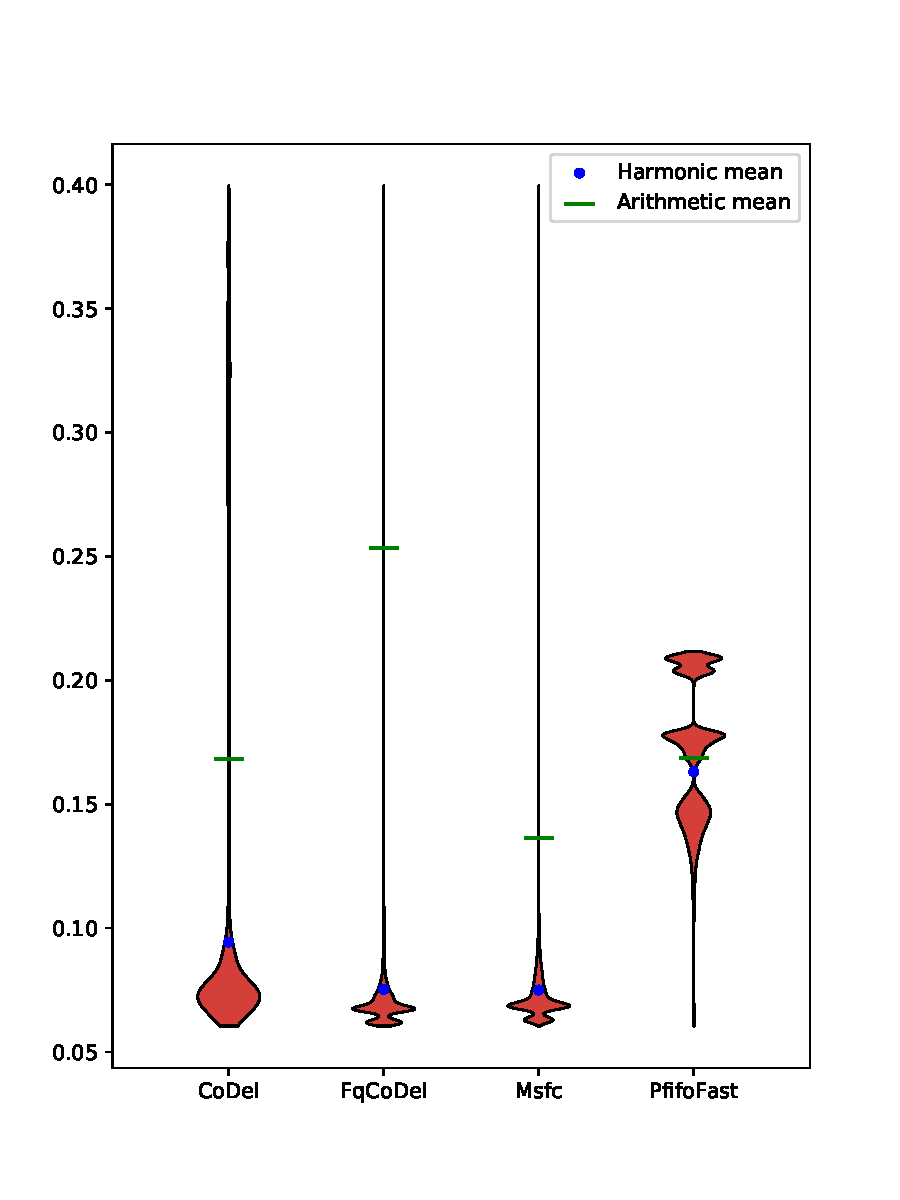
\includegraphics[width=137mm]{drawings/overall-delay-down}
	\caption{The distribution of delay in seconds. Packets with delay higher than 0.4 seconds are omitted in the distribution, but the means are computed from all values. This restriction results in displaying 93\% of data. However, the few packets have such high delay, that it considerably affects the arithmetic means. }
	\label{fig:overall_delay}
\end{figure}

\begin{figure}
	\centering
	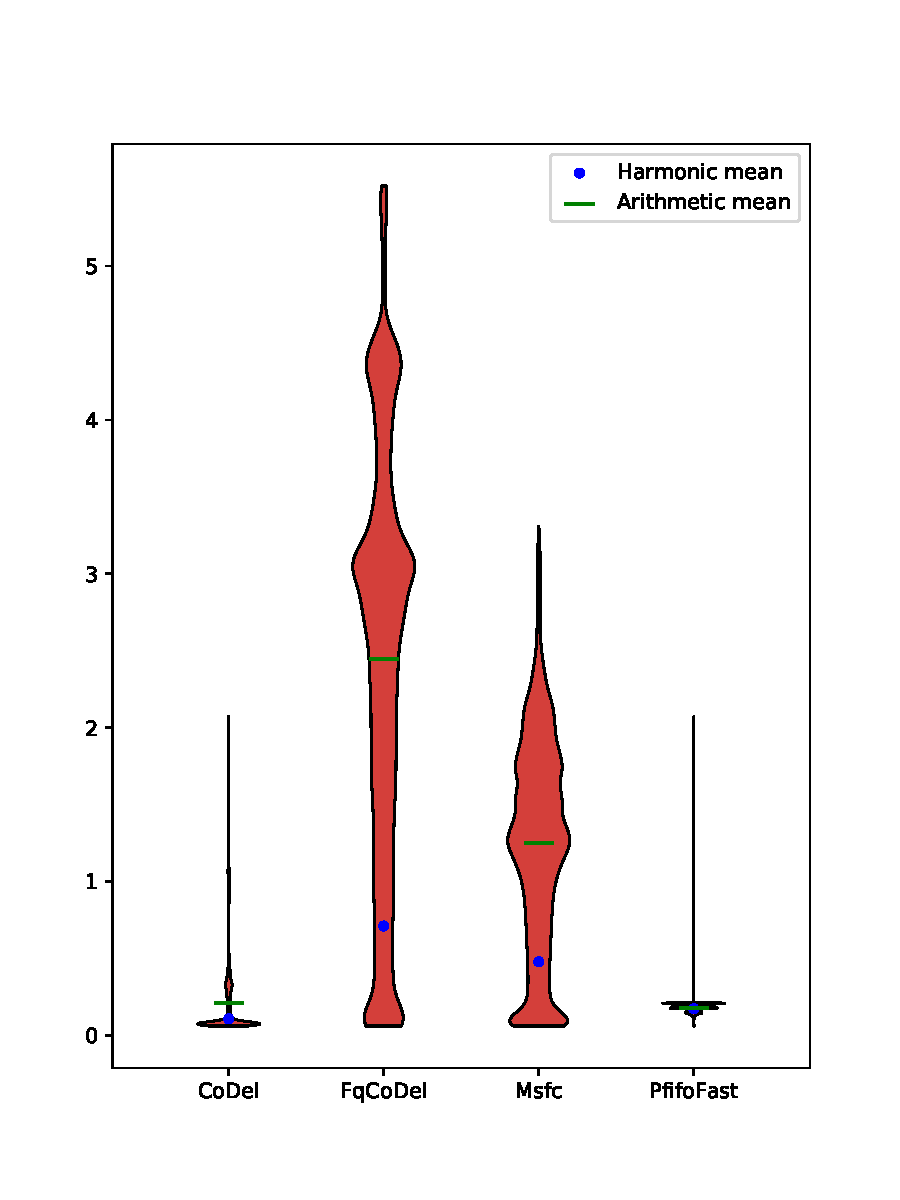
\includegraphics[width=137mm]{drawings/type6-delay-down_A}
	\caption{The distribution of delay of \emph{torrent} packets in seconds in simulation A.}
	\label{fig:torrent_delay}
\end{figure}



\begin{figure*}
	\centering
	\begin{subfigure}[b]{0.475\textwidth}
		\centering
		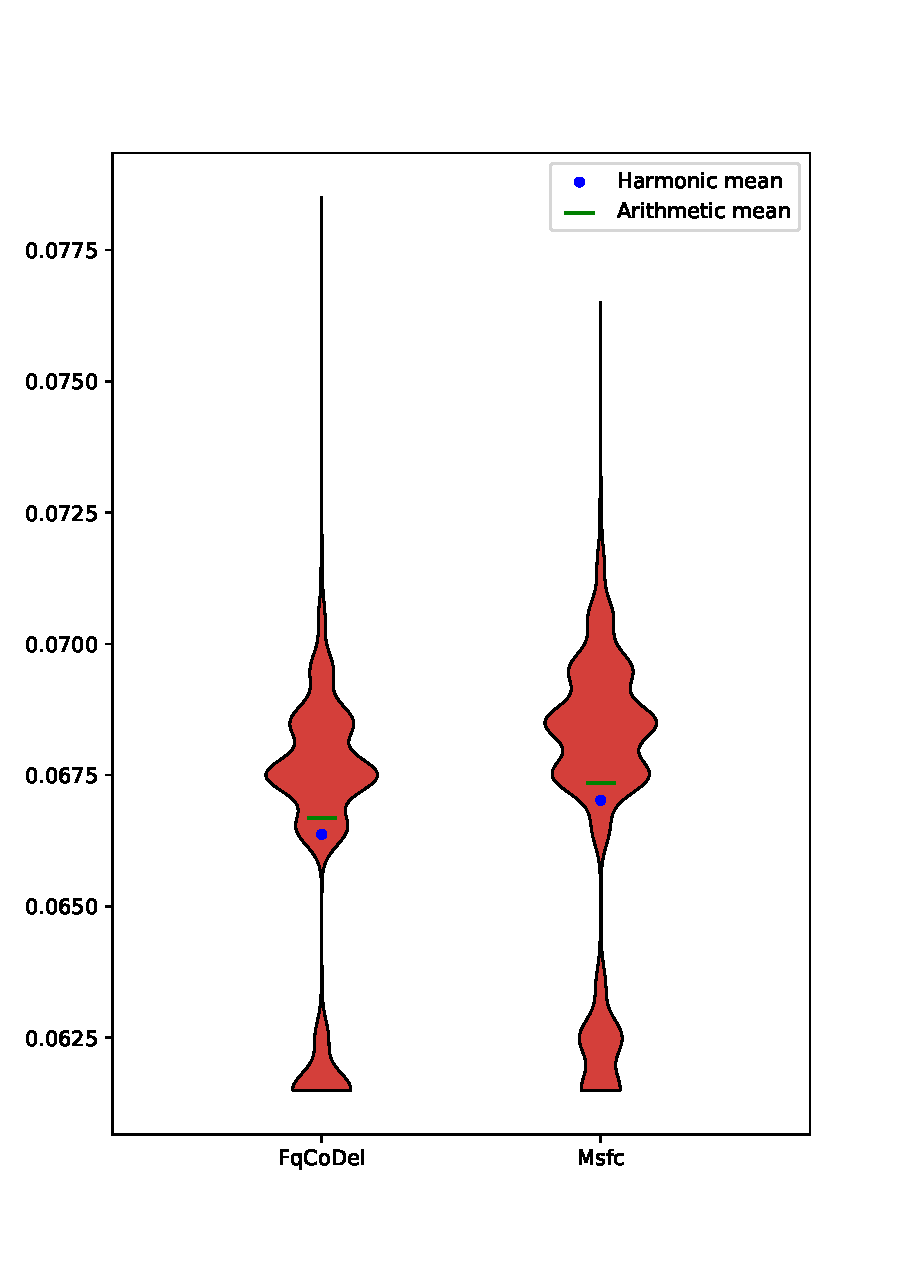
\includegraphics[width=\textwidth]{drawings/type1-delay-down_A}
		\caption[]%
		{{\small Delay of \emph{VoIP} flows}}    
		\label{fig:delay_voip}
	\end{subfigure}
	\hfill
	\begin{subfigure}[b]{0.475\textwidth}  
		\centering 
		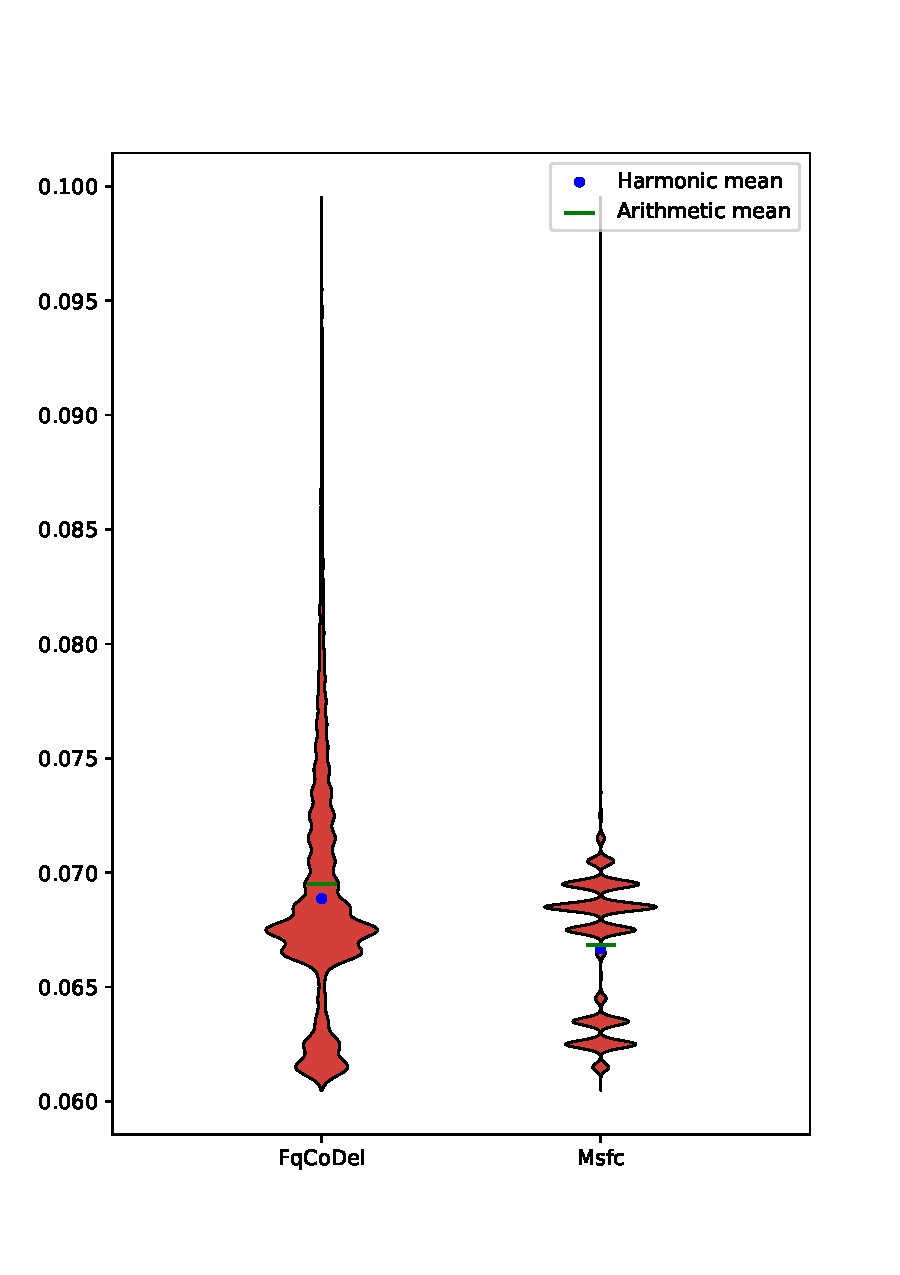
\includegraphics[width=\textwidth]{drawings/type3-delay-down_A}
		\caption[]%
		{{\small Delay of \emph{TV} flows}}    
		\label{fig:delay_tv}
	\end{subfigure}
	\par\bigskip % force a bit of vertical whitespace
	\begin{subfigure}[b]{0.475\textwidth}   
		\centering 
		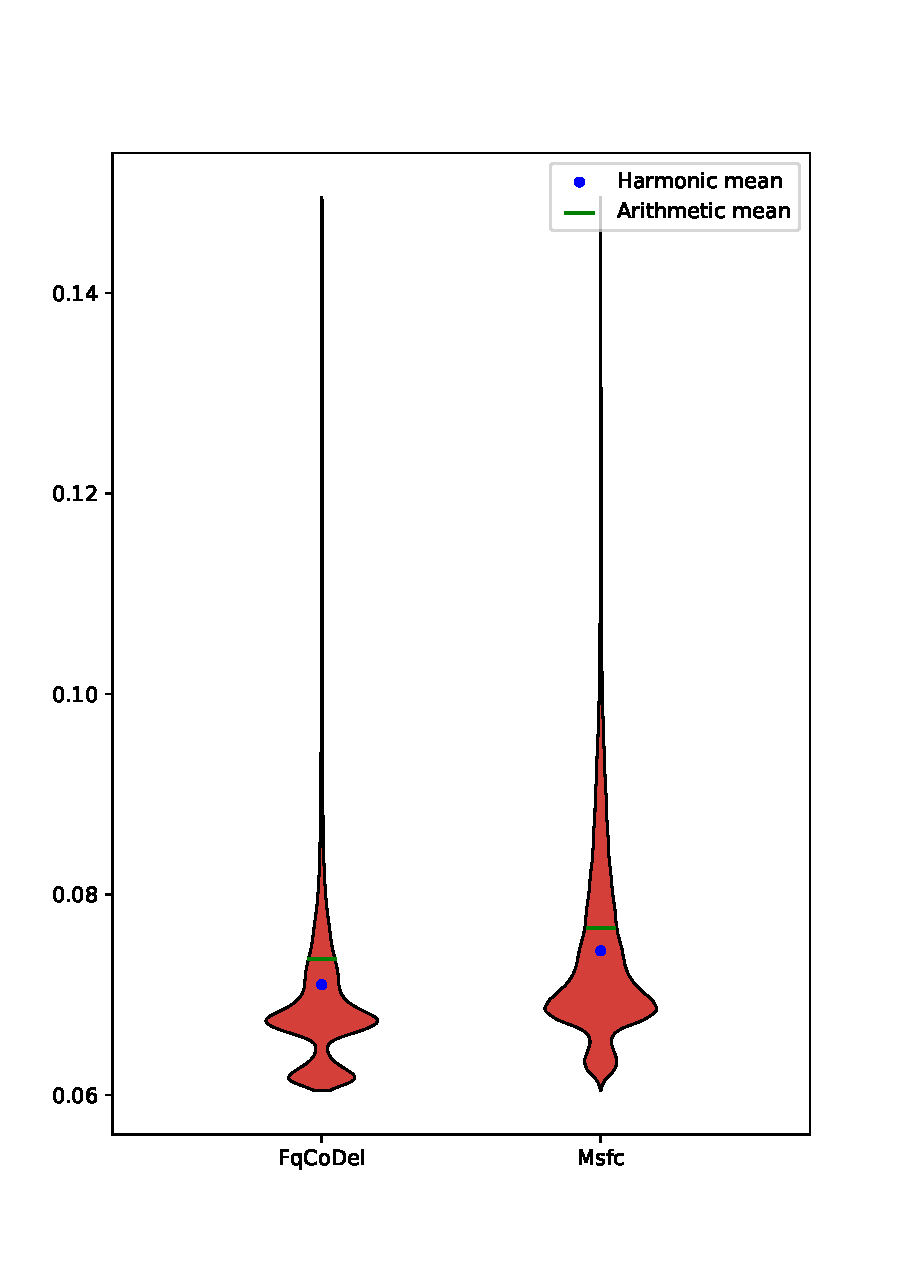
\includegraphics[width=\textwidth]{drawings/type4-delay-down_A}
		\caption[]%
		{{\small Delay of \emph{HTTP} flows}}    
		\label{fig:delay_http}
	\end{subfigure}
	\quad
	\begin{subfigure}[b]{0.475\textwidth}   
		\centering 
		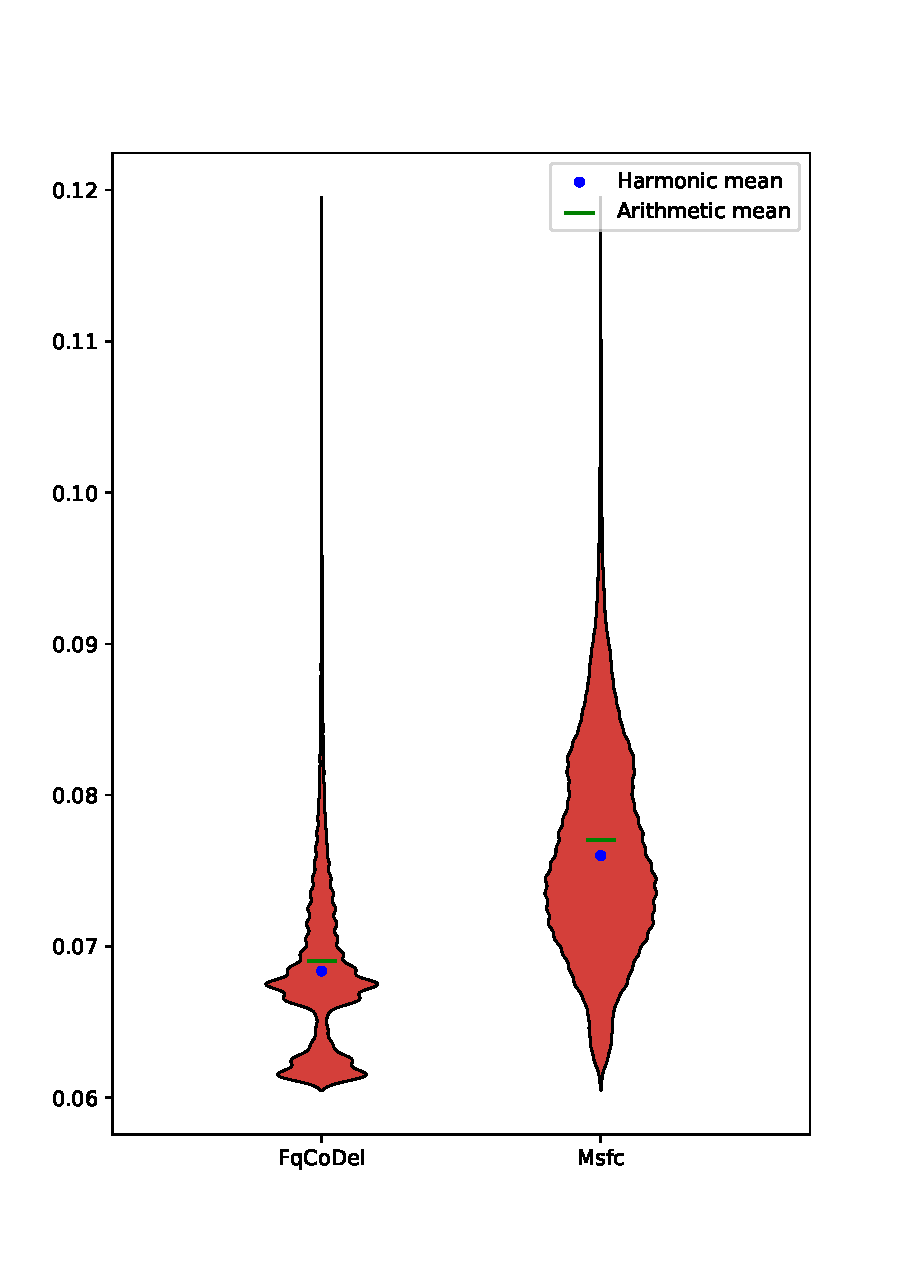
\includegraphics[width=\textwidth]{drawings/type5-delay-down_A}
		\caption[]%
		{{\small Delay of \emph{download} flows}}    
		\label{fig:delay_download}
	\end{subfigure}
	\caption[]
	{\small The distribution of delay of different types of flows. We omit a small fraction of extreme values to get better visualization, however the means are calculated from all values.} 
	\label{fig:delay_flows_A}
\end{figure*}





\clearpage
\section{Traffic distribution caveat}
\todo{ -- ukazujes to jen jako doplnkovou simulaci (ne B) na ktery demonstrujes nebezpeci kdyz hloupej administrator nasype hodne veci do vyssich trid a mysli si ze to necemu pomuze. (Real world experience: lidi vod siti MILUJOU vsemu nastavit nejvyssi prioritu a pak pozorovat jak se to chova uplne stejne a vsem rikat ze to je nejrychlejsi co to de. Kdybys tam chtel nejakej satirickej footnote, tak tenhle, zaslouzej si to. :D)}

\begin{table}
	\caption{Priorities assigned to types of flows and resulting number of flows in simulation B.}
	\label{tab:flows_count_B}
	\centering
	
	\begin{tabular}{@{}l|cccc@{}}
		\toprule
		\multicolumn{1}{c|}{Application} & Priority & \multicolumn{3}{c}{Number of flows}   \\
		\multicolumn{1}{c|}{type}        &          & Priority 0 & Priority 1 & Priority 2  \\ \midrule
		SSH                              &    2     &     0      &     0      &     9       \\
		VoIP                             &    2     &     0      &     0      &     9       \\
		Game                             &    2     &     0      &     0      &     9       \\
		TV                               &    1     &     0      &     27     &     0       \\
		HTTP                             &    1     &     0      &    162     &     0       \\
		Download                         &    1     &     0      &     40     &     0       \\
		Torrent                          &    0     &     24     &     0      &     0       \\ \midrule
		Total                            &          &     24     &    229     &     27      \\ \bottomrule
	\end{tabular}
\end{table}


\XX{In second simulation we demonstrate that assigning the priorities to flows may not be as straightforward as it may seem when using MSFC. We ran the simulation with priorities according to Table \ref{tab:flows_count_B}. The overall results of the simulation are shown in Table \ref{tab:results_B}. The Figure \ref{fig:delay_flows_B} shows distribution of selected types of flows. The performance of all schedulers except MSFC remained unchanged, since MSFC is the only scheduler that takes priorities into consideration.}

The notable difference is noticeable in the throughput of \emph{torrent} flows, see Table \ref{tab:throughput_B}. With this priority assignment, MSFC gave \emph{torrent} almost two times higher throughput than FQ CoDel, although we assigned the lowest priority to the \emph{torrent} flows. All the priority 1 flows have less throughput and worse delay. This unpleasant behaviour is caused by the distribution of flows into the priorities (see Table \ref{tab:flows_count_B}) and the fact, that MSFC treats flows of different priority classes absolutely separately. There are too many flows, that 'fight' for the bandwidth of priority 1 class, while there are few flows, for which MSFC reserves whole priority 0 class.

The priority 2 flows results ended up without any notable difference. Also it is worth mentioning, that even though we assigned flows with low data rate to the priority 2 class, which reserves huge bandwidth, it did not affect the overall throughput negatively. When packets of the highest priority class were not available, its bandwidth was assigned to the rest of priority classes.


\begin{table}[]
	\centering
	\begin{tabular}{@{}lrrrr@{}}
		\toprule
								& CoDel & FQ CoDel & MSFC & pfifo\_fast  \\ \midrule
		Throughput (kbps)       & 290066    & 290264 & 290372   & 290613 \\
		Delay (ms)              & 94.4      & 75.2   & 85.9     & 163.1    \\
		Jitter (ms)             & 0         & 2      & 2        & 0      \\
		Packet Loss (packets)   & 86731     & 1571844& 1180488  & 68259  \\ \bottomrule
	\end{tabular}
	\caption{Overall results of simulation B. The table shows average network throughput in kilobits per second, harmonic mean of packet delay in milliseconds, arithmetic mean of packet jitter in milliseconds and the total number of packets lost.}
	\label{tab:results_B}
\end{table}


\begin{table}

	\centering
	
	\begin{tabular}{@{}l|rrrr@{}}
		\toprule
						& CoDel & FQ CoDel & MSFC & pfifo\_fast  \\ \midrule
		SSH             &     257       &     64        &     64        &     183       \\
		VoIP            &     108       &     66        &     66        &     160       \\
		Game            &     139       &     65        &     64        &     163       \\
		TV              &     124       &     69        &     73        &     155       \\
		HTTP            &     108       &     73        &     75        &     153       \\
		Download        &     105       &     69        &     77        &     150       \\
		Torrent         &     207       &     2448      &     936      &     178       \\ \bottomrule
	\end{tabular}
	\caption{Average delay of individual types of flows in milliseconds in simulation B.}
	\label{tab:delay_B}
\end{table}

\begin{table}
	\centering
	
	\begin{tabular}{@{}l|rrrrr@{}}
		\toprule
		& {CoDel} & {FQ CoDel} & {MSFC} & {pfifo\_fast}  \\ \midrule
		SSH       &    48         &    0          &    0          &    1709  \\
		VoIP      &    167        &    0          &    0          &    311   \\
		Game      &    197        &    3          &    0          &    488   \\
		TV        &    979        &    719        &    1009       &    3124  \\
		HTTP      &    5239       &    3670       &    4187       &    14232 \\
		Download  &    1360       &    1099       &    1440       &    4923  \\
		Torrent   &    78741      &    1566353    &    1173852    &    43472 \\ \bottomrule
	\end{tabular}
	\caption{Number of lost packets by flow types in simulation B.}
	\label{tab:loss_B}
\end{table}

\begin{table}
	\centering
	\begin{tabular}{@{}l|rrrrr@{}}
		\toprule
		         & {Data rate} & {CoDel} & {FQ CoDel} &  {MSFC} & {pfifo\_fast} \\ \midrule
		SSH      &           1 &    3.60 &       3.51 &    3.51 &          3.41 \\
		VoIP     &          60 &   66.47 &      73.04 &   73.02 &         57.47 \\
		Game     &         100 &   80.67 &     107.43 &  107.44 &         66.71 \\
		TV       &        3000 &  270.50 &    1327.67 &  967.26 &        265.41 \\
		HTTP     &   unlimited &  231.41 &     919.32 &  758.23 &        220.30 \\
		Download &   unlimited &  362.88 &    1311.46 &  962.31 &        328.85 \\
		Torrent  &   unlimited & 9558.39 &    2140.52 & 4219.79 &       9727.35 \\ \bottomrule
	\end{tabular}
	\caption{Average throughput of individual flows sorted by flow types in kilobits per second (kbps) in simulation B.}
	\label{tab:throughput_B}
\end{table}












\begin{figure*}
	\centering
	\begin{subfigure}[b]{0.475\textwidth}
		\centering
		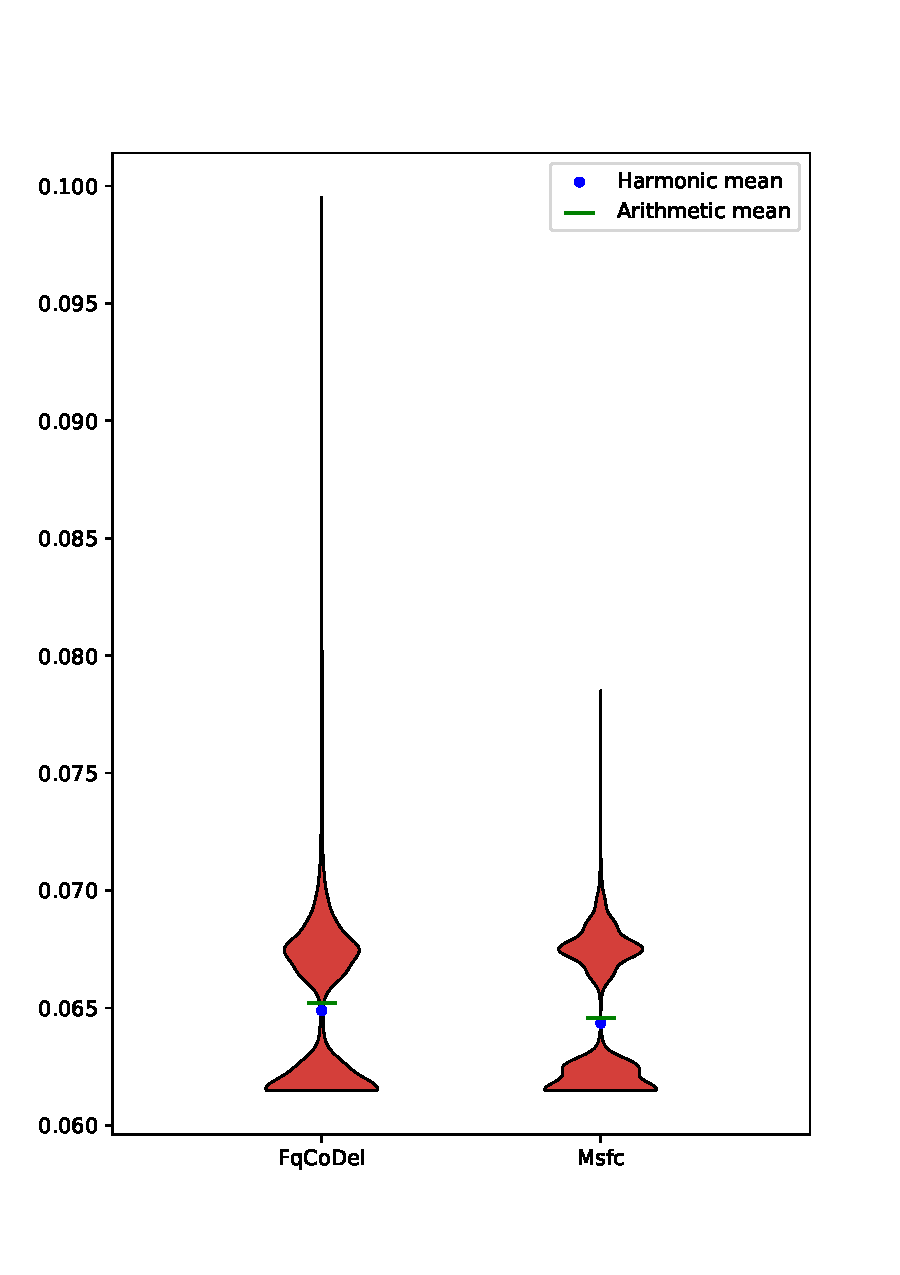
\includegraphics[width=\textwidth]{drawings/type2-delay-down_B}
		\caption[]%
		{{\small Delay of \emph{game} flows}}    
		\label{fig:delay_voip_A}
	\end{subfigure}
	\hfill
	\begin{subfigure}[b]{0.475\textwidth}  
		\centering 
		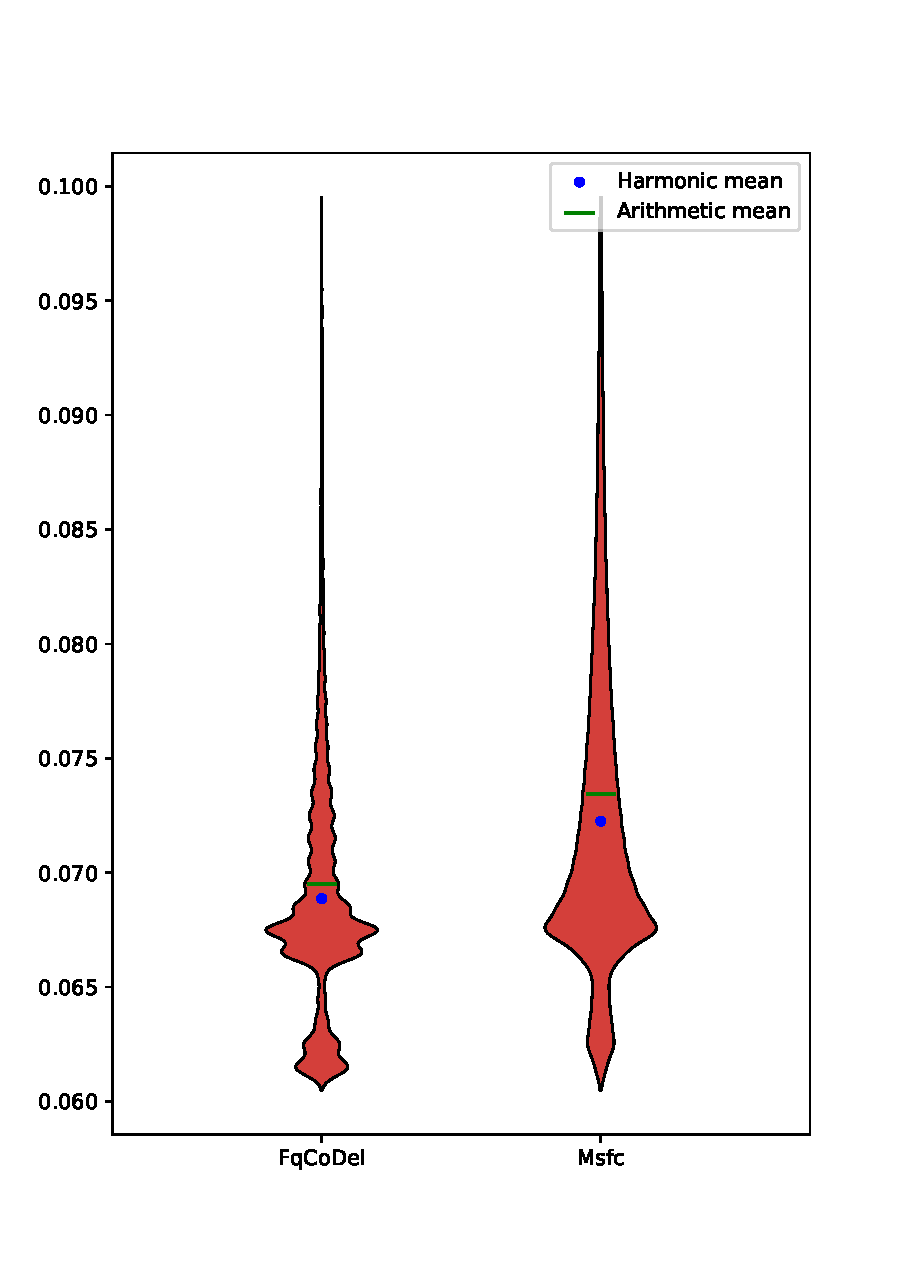
\includegraphics[width=\textwidth]{drawings/type3-delay-down_B}
		\caption[]%
		{{\small Delay of \emph{TV} flows}}    
		\label{fig:delay_tv_B}
	\end{subfigure}
	\par\bigskip % force a bit of vertical whitespace
	\begin{subfigure}[b]{0.475\textwidth}   
		\centering 
		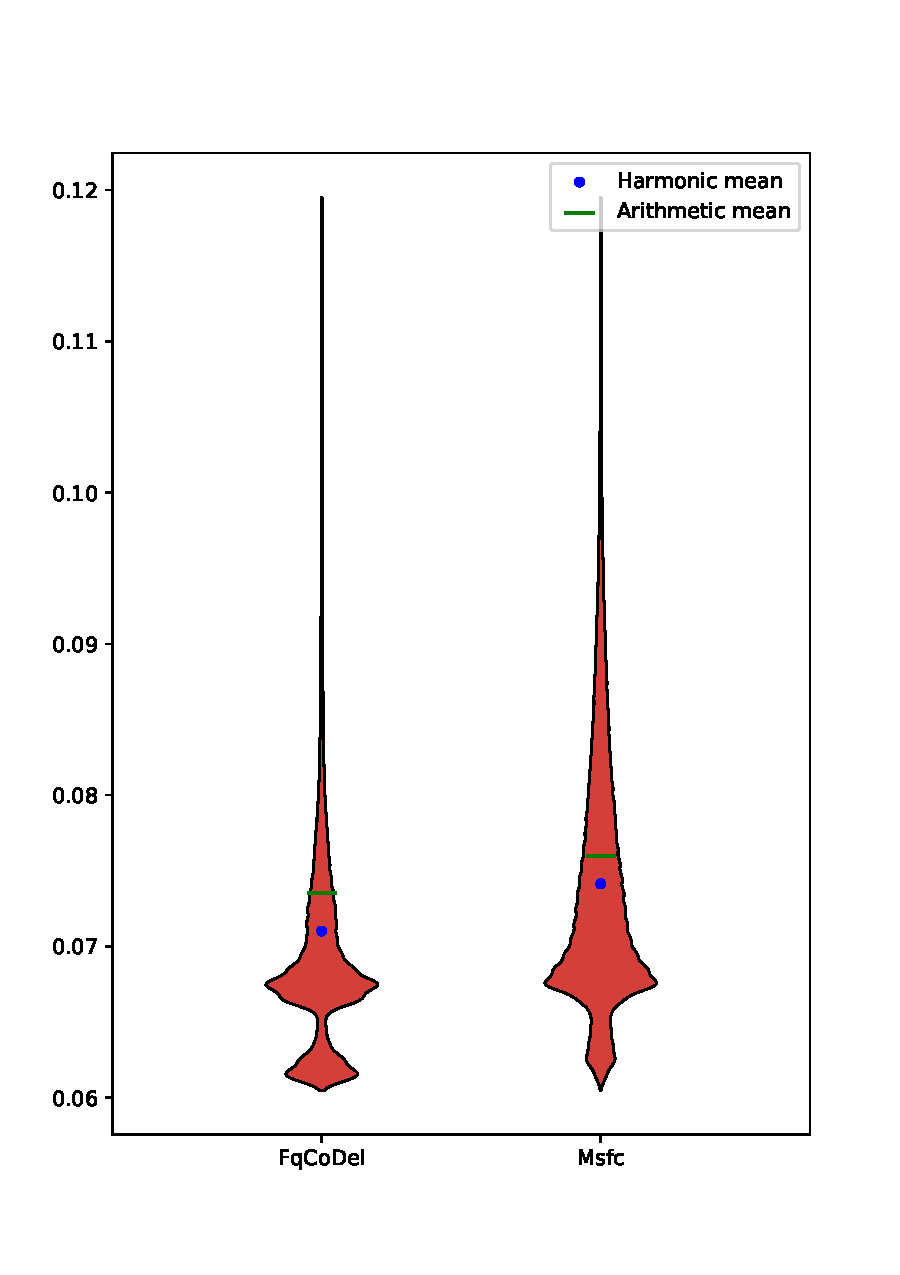
\includegraphics[width=\textwidth]{drawings/type4-delay-down_B}
		\caption[]%
		{{\small Delay of \emph{HTTP} flows}}    
		\label{fig:delay_http_B}
	\end{subfigure}
	\quad
	\begin{subfigure}[b]{0.475\textwidth}   
		\centering 
		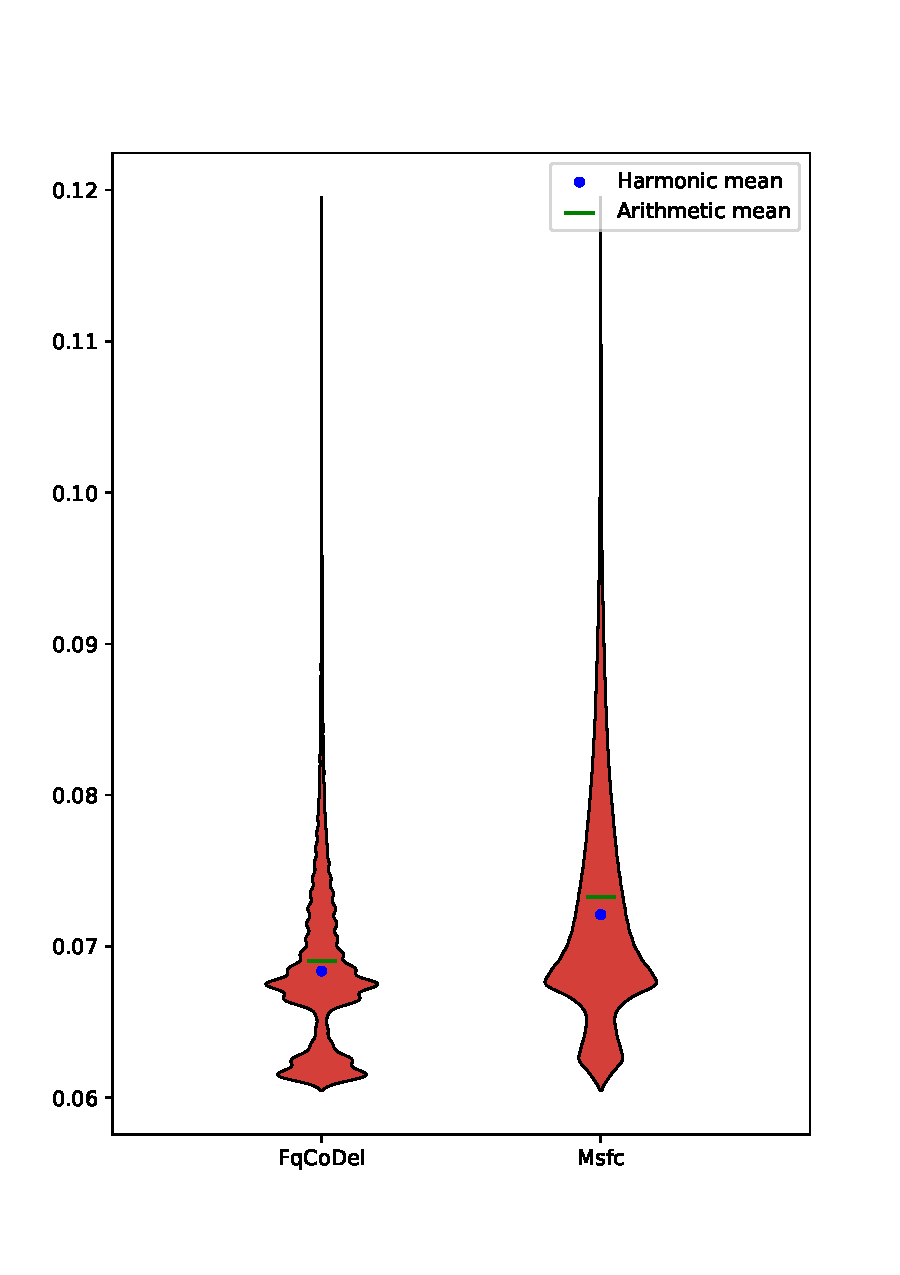
\includegraphics[width=\textwidth]{drawings/type5-delay-down_B}
		\caption[]%
		{{\small Delay of \emph{download} flows}}    
		\label{fig:delay_download_B}
	\end{subfigure}
	\caption[]
	{\small The distribution of delay of different types of flows in simulation B. We omit few extreme values to get better visualization, however the means are calculated from all values.} 
	\label{fig:delay_flows_B}
\end{figure*}



\section{Discussion}

We showed that MSFC can be easily used to prioritize important traffic and services that have high requirements on network resources. The results of simulation A (see Table \ref{tab:throughput_A}) showed, that the prioritized \emph{TV} flows received much more bandwidth, while maintaining other flows' quality of service reasonably. In reality, this can be the difference between working and unusuable internet TV. \todo{v ty tabulkce je dokonce nekde videt ze to u TV uplne odstranilo packet loss! zvyraznit! :D}

\XX{In the simulation B,} presented unintuitive behaviour of MSFC under certain conditions. By design, MSFC reserves certain share of bandwidth to each priority class, regardless of number of flows in each class. This works well one way --- the more precious services are guaranteed to get certain bandwidth, as long as they are relatively rare. In contrast, puting most flows in a higher-priority class effectively causes it to become a `bloated' low-priority class where the services do not prioritize well against each other; moreover, less important or misbehaving flows in the lower priority classes will counter-intuitively receive more bandwidth, because of bandwidth ratio separation in the first layer of MSFC design.

However, with this in mind, MSFC flow classification can still be configured correctly and easily using only a rough estimation of number of flows of different types. Another possibility would be to use more priority classes, so the lowest priority class gets even less bandwidth. Note that other traffic schedulers that allocate bandwidth show similar corner cases with unintuitive behaviour --- one such case can be seen in HFSC \cite[Corner cases section]{hfscMan}.











